%% PNAStwoS.tex
%% Sample file to use for PNAS articles prepared in LaTeX
%% For two column PNAS articles
%% Version1: Apr 15, 2008
%% Version2: Oct 04, 2013

%% BASIC CLASS FILE
\documentclass{pnastwo}

%% ADDITIONAL OPTIONAL STYLE FILES Font specification

%\usepackage{pnastwoF}

\usepackage{xr}
\externaldocument[S]{supp}
\usepackage{dcolumn}
\usepackage{booktabs}

%% OPTIONAL MACRO DEFINITIONS
\def\s{\sigma}
%%%%%%%%%%%%
%% For PNAS Only:
\url{www.pnas.org/cgi/doi/10.1073/pnas.0709640104}
\copyrightyear{2008}
\issuedate{Issue Date}
\volume{Volume}
\issuenumber{Issue Number}
%\setcounter{page}{2687} %Set page number here if desired
%%%%%%%%%%%%

\begin{document}

\title{Hysteresis in human computation:\\ how one task affects another}

\author{Edward Newell\affil{1}{McGill University, School of Computer Science,
Canada}
\and
Derek Ruths\affil{1}{}}

\contributor{Submitted to Proceedings of the National Academy of Sciences
of the United States of America}

%%%Newly updated.
%%% If significance statement need, then can use the below command otherwise just delete it.
%\significancetext{RJSM and ACAC developed the concept of the study. RJSM conducted the analysis, data interpretation and drafted the manuscript. AGB contributed to the development of the statistical methods, data interpretation and drafting of the manuscript.}

\maketitle

\begin{article}
\begin{abstract}

{Microtask platforms are becoming commonplace tools for performing human
research, producing gold-standard data, and annotating large datasets.
These platforms connect \textit{requesters}
(researchers or companies) with large populations (crowds) of workers, who 
perform small jobs, typically taking less than five minutes each.
A topic of ongoing research concerns designing jobs that elicit high 
quality annotations. Here we identify a feature of nearly all crowdsourcing 
jobs that can seriously bias the results produced by workers.  %acts as a strong, systemic source of bias. 
Microtask jobs typically consist of a sequence 
of tasks sharing common format 
(e.g., circle galaxies in an image). 
Using image-labeling, a canonical microtask job format, we 
discover that earlier tasks have a priming effect on the worker, shifting the 
distribution of future answers by 30-50\%. 
Moreover, prior tasks influence the content that workers focus on, 
as well as the richness and specialization of responses. 
Understanding these \textit{intertask effects} is crucial 
to ensuring the utility of microtask platforms in diverse applications.
While intertask effects can be a source of systematic bias, 
our results suggest that, with appropriate job design, 
they might be leveraged to hone worker focus and acuity, 
helping to elicit reproducible, expert-level judgments.} 

\end{abstract}

\keywords{human computing | crowd sourcing | priming}

%\abbreviations{SAM, self-assembled monolayer; OTS, octadecyltrichlorosilane}

\dropcap{M}icrotask platforms are online marketplaces in which \textit{requesters} 
post batches of tasks, and \textit{workers} complete them
for remuneration, a sense of purpose, and fun
\cite{kazai2013analysis}.
Typical tasks include tagging and categorizing images,
%\cite{6116320,Zhai2012357}, 
coding and transcribing media,
%\cite{chandler2013breaking,Berinsky2012351,Finnerty2013},%paolacci2010running}, 
judging the relevancy or quality of content, 
and performing surveys for academic or market reserach purposes (see Table S\ref{Stable:task_composition} for a survey of task types).
%\cite{le2010ensuring,grady2010crowdsourcing,alonso2009can,kazai2013analysis}.

This form of crowdsourcing embeds workers in a controlled but flexible
task infrastructure.  To the requester, workers seem almost like input-output 
devices.  
This provides much of the flexibility and 
cost-savings of fully automating the work in a computer program: 
the workforce is available on demand over the Internet using automated 
scripts, without the need for interviews or contracts 
\cite{wolfson2011look,5543192}.
Jobs can be performed at a fraction of the cost of traditional methods for 
recruiting temporary workers or experimental subjects
\cite{Berinsky2012351}. %,ranade2012crowdsource}%,paolacci2010running}.
Many researchers consider microtask platforms 
as a new kind of \textit{human computing} architecture
\cite{5543192}. %,little2010turkit,minder2012crowdlang,kittur2011crowdforge}.

%The flexibility and cost-effectiveness of microtask labour
%has led to a surge in demand from industry and 
%academia\cite{wolfson2011look,Berinsky2012351}.  More recently, microtask 
%platforms have
%been proposed as a means to use non-specialized workers to supplement expert human resources in critical applications, such as in medical diagnostics,
%with promising results \cite{Warby2014385}.
To be useful, these platforms must be reliable, leading researchers to investigate the factors affecting the reliability
of microtask work, including
the level of pay \cite{Mason200977,kazai2013analysis}, 
the training and pre-screening of workers 
\cite{le2010ensuring,kazai2013analysis}, %paolacci2010running}, 
user-interface design \cite{Finnerty2013}, and the provision of timely 
feedback \cite{Dow20121013}.
Researchers have also investigated \textit{framing}, 
by altering the description of the workflow context 
\cite{Kinnaird2012281}, the stated purpose of tasks 
\cite{chandler2013breaking}, and the problem description
\cite{thibodeau2013natural}.  Another important optimization concerns
workflow design: how breaking down a complex problem into microtasks
\cite{kittur2011crowdforge}, altering microtask size 
\cite{Huang201077}, and introducing workflow interruptions 
\cite{laseckieffects} impact worker quality and efficiency.

Here, we focus on how a ubiquitous feature of microtask work affects reliability. Because tasks are short (hence the term `microtask'), there is a tendency for workers to perform many similar tasks in quick succession.  In fact, on the most popular microtask platform, Amazon's Mechanical Turk (MTurk),
tasks are typically delivered in bundles called HITs.
Although HIT stands for ``Human Intelligence Task'', here we use ``task'' to 
mean the smallest repeatable unit of work.  For example, one HIT may involve 
labeling ten images with descriptive words (\textit{labels}), which amounts
to ten tasks, each being the labeling of a single image.
In addition to the task-repetition occuring \textit{within} HITs, 
workers prefer those HITs that have many available repetitions (that is,
many more HITs of the same format, but with different data) 
\cite{Chilton20101}, probably because performing similar tasks reduces 
cognitive load from task-switching\cite{Adamczyk2004271}.

The repetitive completion of similar tasks is of concern because people's 
responses to a prompt can be strongly influenced by their recent exposure to 
stimuli, due to \textit{priming} 
\cite{BJOP1796}. %,No2007}. %,beller1971priming}.  
Priming can arise when 
a prior stimulus is conceptually or perceptually related to an ensuing 
task, so the repetition of 
similar tasks may create an opportunity for strong priming effects
\cite{Gass1999549}. %,sohn2001task}

%Researchers investigating a somewhat similar class of psychological phenomena,
%found that ratings that microtask workers give to items in a list
%depend on the order in which the list is presented, an effect known as
%\textit{positional bias} \cite{lerman2014leveraging}.  This serves as an 
%example of a basic psychological phenomenon impacting crowdsourced data,
%and raises questions about what other cognitive biases might
%affect microtask work, and how prevalent the induced bias might be.  

Here, we investigate the potential for task repetition to induce bias in 
a highly generalizeable microtask setup, in which workers label a 
series of images.  If task-induced priming arises in this setup, 
it can be expected in virtually every microtask and crowdsourced workflow
where workers are called upon to exercise their judgment.

Our results show that a worker's response during a task
does indeed depend strongly on the tasks performed beforehand.   
We call the effects that earlier tasks exert on later ones 
\textit{intertask effects}.  If, as has been suggested \cite{5543192}, 
microtask platforms are to be considered as a new form of computing 
architecture, it will be necessary to reconcile the fact that the human 
computing elements 
exhibit \textit{hysteresis}, meaning that microtask workers' outputs depend 
on the \textit{history} of their inputs.

\section{Results}

Our image-labeling tasks were performed on the MTurk microtask platform.  We
chose image labeling because it is very common,
%,paolacci2010running},
and because it is prototypical for tasks in which the worker is
asked to provide a response that is not precisely determined by the prompt, but
instead depends on the worker's judgment
\cite{chandler2013breaking,Finnerty2013}.  This includes such diverse tasks as
describing video and audio recordings, summarizing texts, or in clinical
diagnostic judgments.

In our first experiment, called \textit{intertask-food-objects}, workers were
assigned to either a \textit{food} or \textit{objects} treatment.  Workers in
both treatments performed a set of five \textit{initial tasks}, which each
involved providing descriptive labels for an image depicting either food or
(non-food) objects, depending on the worker's treatment (Fig.~\ref{fig:task}A
and B).  Following the initial tasks, workers performed five \textit{test
tasks}, which were identical for both treatments.  In the test tasks, workers
labeled images, each of which depicted a mixture of food and objects
(Fig.~\ref{fig:task}C).  The five initial and test tasks performed by each
worker comprised one HIT. The images were presented one at a time, and we made
no distinction between the initial and test tasks. Finally, workers were only
allowed to participate in one HIT relating to this study, ensuring that prior
exposure to the experiment design and content was not an issue.

The frequencies of words used by workers in the \textit{food} and
\textit{objects} treatments differed significantly during test tasks (by
$\chi^2$ test, $p = 6.0 \times 10^{-14}$), even though the test tasks were
identical in both treatments (see Supplementary Material for tabulated
statistics).  This establishes our most fundamental finding: earlier tasks do affect
later ones. %, raising concerns about the the microtask methodology.

Having affirmed the \textit{existence} of intertask effects, we wish to
understand the nature and severity of the bias induced.  We therefore define
the extent of bias, $\theta$, in terms of the strength of influence that a
prior perturbation has on workers' responses.  Since workers' responses are
stochastic, we define the extent of bias in terms of the change induced in the
distribution of responses:

\begin{equation}
	\theta = \frac{1}{2}\sum_{x \in X} \left| p_0(x) - p_1(x) \right|,
	\label{eq:theta}
\end{equation}

where $p_i(x)$ is the probability that a worker, subjected to treatment $i$,
provides response $x$, from the set of possible responses $X$. This formulation
is a general divergence metric between probability distributions known as the
{\it total variation distance}. Determining $\theta$ from finite samples of
responses, using purely statistical approaches, is difficult (see supplementary
text), which leads us to reformulate the problem in terms of classification:
given a worker's responses to test tasks, can a machine reliably infer what her
prior exposure had been?  Intuitively, the greater the effect that prior tasks
have on subsequent responses, the more accurate the classifier can be.
Formally (as shown in the supplementary material), the accuracy of such a
classifier, $\eta$, establishes a lower bound on the bias:

\begin{equation}
	\theta \geq 2\eta - 1.
	\label{l1}
\end{equation}

By measuring the accuracy of a classifier, we bound the bias induced by a
perturbation, such as the exposure to prior tasks or framing.  Bias ranges from
0 (meaning the exposure does not affect the distribution of responses), to 1
(or 100\%) (meaning that the exposure leads workers to provide a completely
different set of responses).

\begin{figure*}
	\centering
	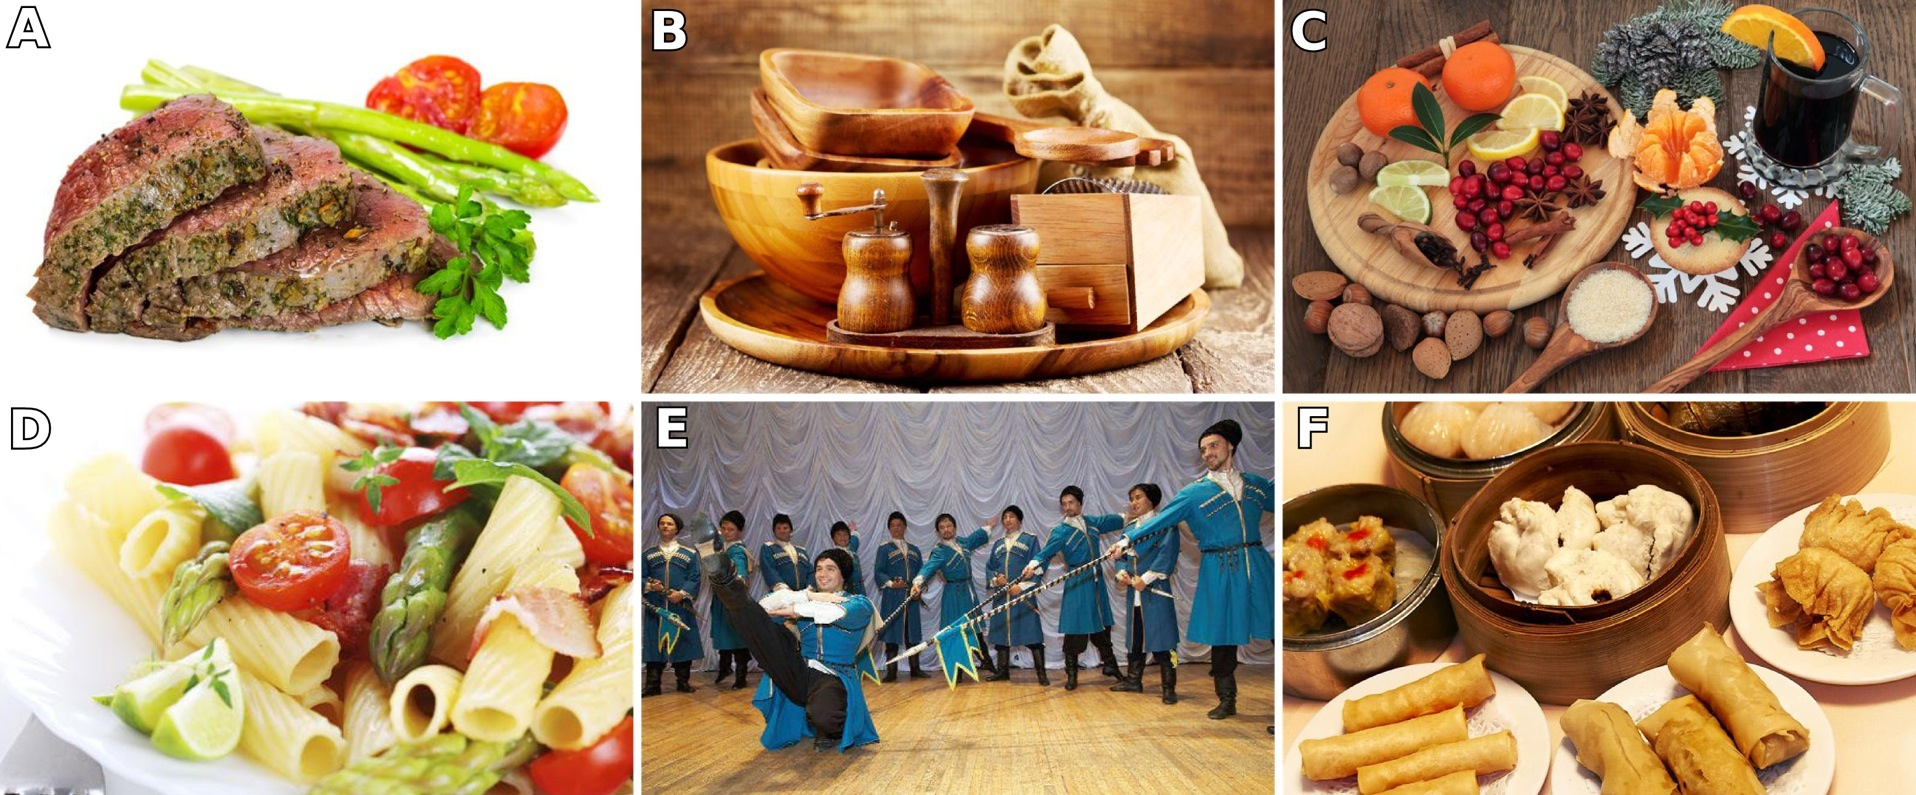
\includegraphics[scale=1.0]{figs/images.jpg}
	\caption{
		Examples of images used in
		initial tasks for the (\textbf{A}) \textit{food} and (\textbf{B}) 
		\textit{objects} treatments of \textit{intertask-food-objects};
		(\textbf{C}) test tasks for \textit{intertask-food-objects} and 
		\textit{frame-food-objects};
		initial tasks for the (\textbf{D}) \textit{food} and (\textbf{E}) 
		\textit{culture} treatments of \textit{intertask-food-culture};
		and (\textbf{F}) test tasks for \textit{intertask-food-culture} and 
		\textit{frame-food-culture}.
		The full set of experimental materials is shown in the 
		supplementary text.
	}

	\label{fig:task}
\end{figure*}

Using a na\"ive Bayes classifier (other classifiers were considered and tested,
see SM), we found that intertask effects lead to {\it at least} a 30\% bias between workers
from the \textit{food} and \textit{objects} treatments (Fig.~\ref{fig:theta}A).
This represents a substantial potential to distort microtask data.

Of course, intertask effects are not the only means of introducing bias into
worker responses. In particular, there has been considerable interest in the effects that
framing can have on microtask responses
\cite{Kinnaird2012281,chandler2013breaking,thibodeau2013natural}. Therefore, as a point of
comparison, we conducted an experiment, similar to the first, in which we
framed the purpose of the tasks.  In this experiment, called
\textit{frame-food-objects}, the same test-tasks were used, but rather than
exposing workers to initial tasks, workers were either told that the tasks were
``Funded by the laboratory for the visual perception of Food and Ingredients'',
or ``\ldots of Objects and Tools''.  Framing did induce changes in the
frequencies of word usage at significance (as determined by $\chi^2$ test;
$p=0.0012$), but the \textit{extent} of framing-induced bias was not
statistically distinguishable from zero ($p =0.37$) (Fig.~\ref{fig:theta}A),
and was much weaker than the bias due to intertask effects ($p=2.1\times
10^{-5}$).

\begin{figure}
	\centering
	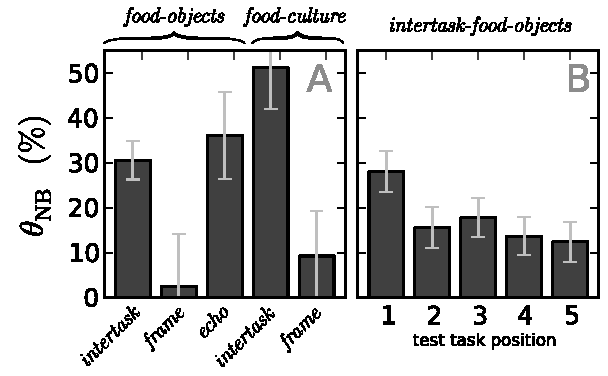
\includegraphics[scale=0.8]{figs/theta.pdf}
	\caption{
		Empirical bias, $\theta_\mathrm{NB}$, measured using a na\"ive Bayes 
		classifier, induced in image labeling tasks, due to workers' 
		exposure to framing and initial tasks.  
		(\textbf{A}) Exposing workers to initial tasks induces more severe
		bias than framing, except when echoed framing is used. 
		(\textbf{B}) As workers proceed through test tasks, 
		the bias due to initial tasks wanes, 
		but remains significant even after five tasks.  
		Standard error bars are shown.
	\label{fig:theta}
	}
\end{figure}

To assess the persistence of intertask effects, we replicated the experiment
\textit{intertask-food-objects} while permuting the test tasks, to reveal the
dependence of intertask effects on task position.  We found that, as expected,
bias was strongest for the first test task (about 28\%), but remained
significant through all five test tasks ($\alpha=0.05$) sustaining over 12\%
bias even when the initial and test tasks were separated by four intervening
tasks (Fig. \ref{fig:theta}B).

We conducted variants of these experiments using different images, to see
whether this trend was robust.  In the experiment
\textit{intertask-food-culture}, workers were either assigned to a
\textit{food} or \textit{culture} treatment.  The initial tasks contained
either images depicting food (Fig.~\ref{fig:task}D), or depictions of cultural
scenes (of dance, sport, or music) (Fig.~\ref{fig:task}E).  The test tasks,
which were, again, identical for both treatments, depicted meals of
identifiable cultural origin (Fig.~\ref{fig:task}F).  As an aside, we recognize
that, despite efforts to the contrary, initial tasks in the food treatment of
\textit{intertask-food-culture} are arguably still of identifiable cultural
origin, but this fact would only tend to make our results more conservative (we
discuss this further in the supplementary text). 

Results for this experiment again showed a strong bias as a result of intertask
effects (about 50\%) (Fig.~\ref{fig:theta}A).  Again, comparing intertask
effects to framing, the experiment (\textit{frame-food-culture}) used the same
test tasks as in \textit{intertask-food-culture}, but exposed workers to
statements framing the purpose of the tasks as the recognition of either food
or culture.  Again, we found that framing effects were weaker than 
intertask effects ($p=7.6\times10^{-7}$).  In fact, framing did not induce 
significant changes in word frequencies (by $\chi^2$ test, $p=0.29$) 
(Fig.~\ref{fig:theta}A).

It was only when framing was combined with an active reiteration step, that
bias reached a comparable extent to that induced by intertask effects.  In the
experiment \textit{echo-food-objects}, after framing the purpose of the task
(as the recognition of food or objects), workers were asked to echo the purpose
of the task using a combo-box input.  This  ``echoed framing'' induced a bias
of about 35\% (Fig.~\ref{fig:theta}A). However, it is difficult to say whether
this should be considered as a framing treatment \textit{per se}: requiring the
worker to reiterate the purpose signals our intent, as the requester, to ensure
that the worker has taken note of it, possibly leading the worker to interpret
the exchange as an instruction.  In any case, it is remarkable that intertask
effects were on par with an explicit, actively reinforced statement of the
tasks' purpose.

% Specificity
To better understand the nature of intertask effects, we investigated the
vocabulary that workers used to label test tasks. One might expect that, within
a given experiment, those workers exposed to food (whether through framing or
initial tasks) would label test tasks using food-related words more often.
Food-related words in labels were identified using the wordnet corpus,
augmented with additional words obtained by crawling a recipe website (see
supplementary text for details).  Surprisingly, we discovered that food-primed
workers typically did not use food words more often. In
\textit{intertask-food-culture}, food-exposed workers actually used
significantly \textit{fewer} food-related words during test tasks
(Fig.~\ref{fig:specificity}A).  This finding rules out the seemingly-simple and
intuitive idea that workers emphasize content that has been present in earlier
tasks: seeing content influences, but does not necessarily \textit{increase},
the probability of referring to it in subsequent tasks.

\begin{table*}[b]
	\centering
	\setlength{\tabcolsep}{4pt}
	\begin{tabular}{ c c c c c }
	
		\setlength{\tabcolsep}{4pt}
		\begin{tabular}{ r | c }
		\toprule
		\multicolumn{2}{c}{
			\parbox[c]{2.5cm}{
				\centering
					\textit{intertask-food-objects}
			}} \\
		\midrule
		coffee & 38 \\
		meal & 34 \\
		cheese & 34 \\
		apple & 32 \\
		dessert & 21 \\
		cup & -30 \\
		glass & -45 \\
		table & -70 \\
		candle & -74 \\
		food & -80 \\
		\bottomrule
		\end{tabular}

&

		\setlength{\tabcolsep}{4pt}
		\begin{tabular}{ r | c }
		\toprule
		\multicolumn{2}{c}{
			\parbox[c]{2.5cm}{
				\centering
				\textit{frame-food-objects}
			}
		}\\
		\midrule
		bread & 18 \\
		wine & 18 \\
		cheese & 16 \\
		apple & 14 \\
		oil & 12 \\
		table & -9 \\
		meal & -10 \\
		candle & -12 \\
		dinner & -13 \\
		food & -32 \\
		\bottomrule
		\end{tabular}

&

		\setlength{\tabcolsep}{4pt}
		\begin{tabular}{ r | c }
		\toprule
		\multicolumn{2}{c}{
			\parbox[c]{2.3cm}{
				\centering
			\textit{echo-food-objects}} 
		}\\
		\midrule
		apple & 24 \\
		cheese & 23 \\
		wine & 15 \\
		coffee & 14 \\
		oil & 7 \\
		knife & -24 \\
		dinner & -26 \\
		fork & -27 \\
		candle & -35 \\
		food & -55 \\
		\bottomrule
		\end{tabular}

&

		\setlength{\tabcolsep}{4pt}
		\begin{tabular}{ r | c }
		\toprule
		\multicolumn{2}{c}{
			\parbox[c]{2.5cm}{
				\centering
			\textit{intertask-food-culture}} 
			\smallskip
		}\\

		\midrule
		spicy & 26 \\
		sauce & 17 \\
		indian & 15 \\
		buffet & 14 \\
		exotic & 12 \\
		festival & -11 \\
		offering & -12 \\
		statue & -15 \\
		india & -20 \\
		food & -56 \\
		\bottomrule
		\end{tabular}

&

		\setlength{\tabcolsep}{4pt}
		\begin{tabular}{ r | c }
		\toprule
		\multicolumn{2}{c}{
			\parbox[c]{2.5cm}{
				\centering
			\textit{frame-food-culture}} 
		}\\
		\noalign{\smallskip}
		\midrule
		indian & 11 \\
		banquet & 8 \\
		spicy & 7 \\
		asian & 6 \\
		variety & 6 \\
		delicious & -6 \\
		meat & -7 \\
		festival & -7 \\
		spice & -7 \\
		food & -9 \\
		\bottomrule
		\end{tabular}

	\end{tabular}
	\caption{
		The five words whose frequencies increased, and those whose 
		frequencies decreased, the most, between treatments of given 
		experiments.  The label frequencies shown apply to the first test
		task.  Positive values indicate that the food-exposed treatment
		used the word with higher frequency.  
		Note that the word ``food'' is always the most suppressed among
		food-exposed workers.  Word frequencies for 
		\textit{intertask-food-objects} correspond to the labels attributed
		to image 1 (see Fig. \ref{Sfig:task1:test}) which is not necessarily 
		the first 
		test task due to the tasks being permuted.  There were five times
		as many workers in \textit{intertask-food-objects}, hence
		larger absolute differences are observed.
	}
	\label{table:top-words}
\end{table*}

To deepen our understanding, we investigated workers' lexical richness in
reference to food, that is, the number of \textit{unique} food-related words
used.  Even if workers provide an abundance of food-related words, there can be
less diversity, if, for example, workers repeat generic references to food.
Both \textit{intertask} experiments showed that food-exposed workers had
greater lexical richness, in reference to food, than their counterparts (as
much as 20\% more) (Fig.~\ref{fig:specificity}B).  This is particularly
noteworthy in the experiment \textit{intertask-food-culture}, because there,
food-primed workers made fewer total references to food.  

The observations regarding lexical richness suggest that initial tasks might
influence workers to use more refined or specialized words, when referring to
aspects of content that had been present in the initial tasks.  To test this,
we used the wordnet corpus to operationalize the notion of word specialization.
Wordnet establishes relationships between 117,798 English nouns, indicating
which words are specializations (or generalizations) of others
\cite{felbaum1998wordnet}.  For example, ``pumpernickel'' is a specialization
of ``bread''.  Within each experiment, we determined the percent-excess of
food-related words that were more specialized in the food-exposed treatment
relative to the other treatment (details in the supplementary material).

In all experiments except \textit{frame-food-culture} (which had only a weak
priming effect), food-primed workers used significantly more
specialized words, in reference to food (about 15\% more)
(Fig.~\ref{fig:specificity}C).  It is interesting that such substantial
increases in both the lexical richness and specialization of food-related words
held for \textit{intertask-food-culture}, where, as mentioned, we observed that
food-exposed workers made \textit{fewer} references to food overall.  These
observations point to countervailing factors: one factor tending to activate
the more specialized and less common food-related words (yielding greater
lexical richness and specialization), and the other tending to suppress
certain, presumably more common and generic words (yielding fewer food-related
words in total).


This hypothesis is corroborated when we look at those words whose frequencies
changed the most from one treatment to another (Table~\ref{table:top-words}).
As one would expect, references to objects, such as ``candle'', ``fork'', 
or ``statue'' appear less frequently among the labels provided by workers in 
food-exposed treatments.  But, the food-exposed workers also provide the most
generic references to to food less often, such as the word ``food'' itself, 
or ``meal''.  
In fact, the word ``food'', which is the most generic possible food-related 
word, was always \textit{the most suppressed} among food-primed workers, 
relative to their non-food-primed counterparts.  
Meanwhile, food-exposed workers provide more specific references to food more 
often, such as ``coffee'', ``cheese'', or ``wine''.


Our results can be explained through a combination of positive and negative
priming.  Positive priming (usually simply ``priming'') occurs when a prior
stimulus predisposes a person to give certain responses in an ensuing task, and
is often observed as an increase in the speed or accuracy of a response, or the
ability to recognize briefer or noisier stimuli
\cite{BJOP1796,BJOP1826,Huber2008324}.  Negative priming occurs when, after
exposure to a stimulus considered to be non-salient, subsequent recognition of
the stimulus is inhibited \cite{mayr2007negative}.

Workers exposed to images containing food are (positively) primed, activating
memories, concepts, and vocabulary related to food.  However, if the worker
labels several images containing food, the basic fact that an image contains
food will not seem salient, since it does not distinguish one image from
another.  Thus, the most generic references to that fact, such as the label
``food'', will be suppressed, while more specialized references will be
elicited.  Meanwhile, the number of references to food overall might increase
or decrease, depending on the balance of these factors.  

More generally, we are suggesting that, even though workers are not instructed
to compare tasks in any way, prior tasks form a context relative to which
workers judge salience.  Thus, due to a combination of negative and positive
priming, a worker's focus in repeated tasks tends to be directed away from
generic, shared features, toward specific and distinguishing ones.

\begin{figure}[t]
	\centering
	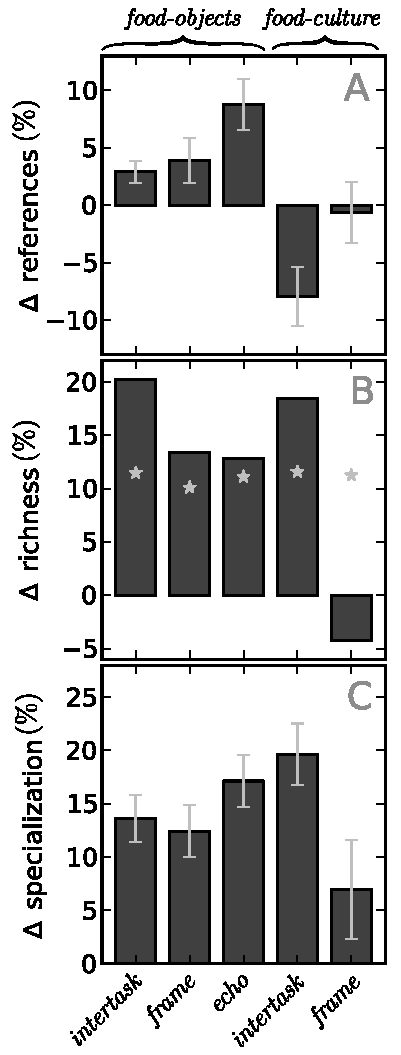
\includegraphics[scale=0.87]{figs/vocab_specificity.pdf}
	\caption{
		Exposing workers to a priming concept, e.g. food, through
		initial tasks or framing, affects their tendency to focus
		on that concept, and the richness and specialization of their 
		vocaubulary in reference to it.
		In all three plots, positive values indicate a larger quantity for 
		the food-exposed workers.
		(\textbf{A}) Exposing workers to food does not necessarily increase
		the fraction food references they provide during test tasks.
		(\textbf{B}) The number of unique food-related
		words (richness) was greater for food-exposed workers, except in the 
		case of \textit{frame-food-culture} (stars indicate the threshold
		for a significant deviation, $\alpha=0.05$). 
		(\textbf{C}) Food-exposed
		workers used more specialized words to refer to food (see 
		supplementary text for calculation of relative specialization).
		Standard error bars are shown in (\textbf{A} and \textbf{C}).
	}
	\label{fig:specificity}
\end{figure}

\section{Discussion}

Prior to this study, little thought appears to have been given to earlier tasks
as a priming vector for later tasks.  But our findings show this is an
important design consideration. 

Our most urgent discovery is that a severe bias can be introduced into
microtask responses, simply from the performance of earlier tasks.  These
effects are much stronger than those of framing. This result impacts a
staggering number of crowdsourcing studies that have been, are currently being,
and will be done.  One approach to minimizing bias could be to randomize task
ordering. This is, in fact, common practice among the crowd sourcing
community already.  Our results, however, indicate that this is an unreliable fix
at best: the sheer magnitude of bias we observed suggests that random ordering
can still admit a significant amount of noise.  Even chains of two or three
similar tasks, which will not be reliably eliminated in random permutations,
could lead to levels of bias like those we observed in our experiments.
Preferably, a deeper understanding of intertask effects might allow them to be
properly controlled.

If controlled in the right way, our findings actually suggest that careful task
engineering might be able to leverage intertask effects to achieve higher 
quality and greater reproducibility in crowdsourcing tasks.  A consistent goal
in human computation is the achievement of expert-level judgments from
non-expert workers \cite{kittur2011crowdforge}.  This has been achieved in some
applications \cite{snow2008cheap,Mortensen20131020,Warby2014385}.  The
distinction between experts and novices is partly attributable to specialized
knowledge and heuristics.  But experts also simplify tasks by more efficiently
directing their focus toward salient features \cite{kellman2009perceptual}.
Our discovery that inter-task effects can produce levels of specificity in
labels indicate that, using strategic task exposure, it might be possible to
guide workers' focus and salience attribution, enabling expert-level judgment
in a wider variety of crowdsourced applications.  We anticipate future work
will yield techniques to control intertask effects, to reduce unwanted bias,
and to tune the focus, diversity, and specificity of worker responses.

Fundamentally, while our findings raise serious concerns about the current
state of microtask design, they also reveal potential opportunities to refine
worker focus and acuity.  Any application that relies on the repetitive use of
human judgment is likely subject to the phenomena described here.  Exploring
the pitfalls and opportunities posed by intertask effects is an important
direction for future work, in the effort to develop more performant and
reliable human computation systems.

\begin{materials}

\section{Microtask setup} This study involved six experiments involving HITs
(bundles of tasks) performed on Amazon's Mechanical Turk (MTurk) platform.  The
flow of events experienced by a worker when participating in this study is
depicted in Fig.~S\ref{Sfig:task_schematic}.  Each experiment was divided into
two treatments.  Treatments for a given experiment differed with respect to a
particular priming modality, which served as the independent variable (as
specified in Table~S\ref{Stable:experiments}).  The HITs for treatments of the
same experiment always involved the same test tasks (the last five tasks in the
HIT), the results of which served as the dependent variable.

All HITs were presented as a series of slides.  The first slide consisted of a
brief set of instructions.  For HITs that included framing, a framing statement
was shown on a slide immediately after the instructions (Fig.
S\ref{Sfig:hit_preamble}B and C).  Initial tasks, when included, followed next.
The initial tasks consisted of a series of five slides, each containing an
image-labeling task like the one shown in Fig.~S\ref{Sfig:hit_preamble}D.
Finally, for all HITs, five slides were shown containing test tasks, in the
same format as the initial tasks.

Workers were randomly assigned to the treatments, and a given worker could only
complete one HIT related to this study.  In \textit{intertask-food-culture},
the \textit{food} and \textit{culture} treatments were both divided into five
sub-treatments, in which the test tasks were permuted.  The permutations were
obtained by rotating the order shown in Fig.~S\ref{Sfig:task1:test} by different
amounts.  For example, rotating by one position involves moving the first image
to the second position, the second image to the third position, and so on, and
moving the last image to the first position.  The five different possible
rotations were used for the five sub-treatments.  This enabled us to study the
effects on each image when it occurred in different positions relative to the
initial tasks.

\section{Selection of images} The images used in the initial tasks for
\textit{intertask-food-objects}  are shown in Figs.~S\ref{Sfig:task1:food}
(\textit{food} treatment) and S\ref{Sfig:task1:obj} (\textit{objects}
treatment).  We took care to exclude objects from the food-images (except for
the dish supporting the food in some cases), and to exclude food from the
object-images.  The images used for the test tasks of
\textit{intertask-food-objects} and \textit{frame-food-objects} are shown in
Fig.~S\ref{Sfig:task1:test}.

The images used in the initial tasks for \textit{intertask-food-culture} are
shown in Figs.~S\ref{Sfig:task2:food} (\textit{food} treatment) and
S\ref{Sfig:task2:cult} (\textit{culture} treatment).  We selected the initial
images for the treatments of this experiment to respectively depict
food and culture.  Naturally, since food is a very important aspect of culture,
pictorial depictions of the two concepts cannot be cleanly separated, and
images depicting food inevitably also depict culture.  However, the fact that
the images for the initial tasks in the \textit{food} treatment of
\textit{intertask-food-culture} also depict culture will only tend to make the
\textit{food} and \textit{culture} treatments more similar.  This would tend to
reduce the severity of intertask effects, but we nevertheless still observed
strong intertask effects.  Thus, the presence of culture in the food-related
initial images of \textit{intertask-food-culture} does not seem to have been
problematic.  The images used in the test tasks of
\textit{intertask-food-culture} and \textit{frame-food-culture} are shown in
Fig.~S\ref{Sfig:task2:test}.

\section{Framing} We framed tasks by including a message, near the beginning
of the HIT, that suggested a particular purpose for the tasks.  The precise
language used is shown in Table~S\ref{Stable:experiments}, and an example of a
framing slide is shown in Fig.~S\ref{Sfig:hit_preamble}B and C.  In
\textit{frame-food-objects} and \textit{frame-food-culture}, the framing
language was based on naming the (fictitious) entity running the study, for
example ``The Global Foundation for the Recognition of Cultures'', or
``Laboratory for the visual perception of Objects and Tools''.  In
\textit{echo-food-objects}, we stated the purpose explicitly (``The purpose of
this task is \dots''), and then required the worker to echo back the purpose of
the task by selecting it from a combo box Fig.~S\ref{Sfig:hit_preamble}C.

In \textit{frame-food-objects} and \textit{echo-food-objects}, we did not
include any initial tasks, meaning that the test tasks followed the framing
slide immediately.  One could argue that a fairer comparison would be achieved
by including initial tasks even for framing experiments (but keeping the
initial tasks constant while varying the framing language), since the worker
would be ``warmed up'' before performing the test tasks, as is the case for the
experiments investigating the effect of initial tasks.  We therefore adopted
this approach in the experiment \textit{frame-food-culture}, in which workers
performed the same initial tasks containing images that depicted food in both
the \textit{food} and \textit{culture} treatments.  It would seem that the
framing effect in \textit{frame-food-culture} was reduced by the initial tasks,
possibly because intertask effects tend to override framing. Further
experimentation would be necessary to be sure, but this was not the purpose of
our study.

\section{Derivation of bias inequality}
A sketch of the derivation of the lower bound on the degree of bias 
$\theta$ in terms of the observed accuracy of a classifier, $\eta$, follows
(see the supplementary material for a detailed derivation). 
Consider the accuracy of the best possible classifier, $\eta^*$.  
Assume two groups of workers, have been
exposed to different treatments, 1 and 2, and as a result have
a different probability of yielding response $x$ during a task: 
$p_1(x)$ and $p_2(x)$.  Upon observing response $x$, it is optimal to guess 
that the worker came from the treatment that produces response $x$ more 
often: i.e. to guess $z=\arg\max_z(p_z(x))$.

The probability that this guess is correct is:
\begin{align}
	\Pr\{\mathrm{correct}\vert x\} 	&= \frac{1}{2} + \frac{|p_0(x) - p_1(x)|}{2 \big(p_0(x) + p_1(x) \big)}.
\end{align}
The probability that the optimal classifier will be correct in general,
which is by definition $\eta^*$, can be found by summing over all possible
responses $x \in \mathcal{X}$:

\begin{align}
	\eta^* &= \sum_{x \in \mathcal{X}} \mathrm{Pr}\{\mathrm{correct}\vert x\}
			\mathrm{Pr}\{x\} \\
		&= \sum_{x\in X} \left(
				\frac{1}{2} + 
				\frac{|p_0(x) - p_1(x)|}{2 \big(p_0(x) + p_1(x) \big)}
			\right)
			\left(
				\frac{p_0(x) + p_1(x)}{2}
			\right)\\
		&= \frac{1 + \theta}{2}
\end{align}

Since no classifier can be more accurate than the optimal classifier, we 
obtain the bound stated in Eq.~\ref{l1}.

\end{materials}

\begin{acknowledgments}
This work was partially supported by an Insight Grant from the Canadian Social Sciences and Humanities Research Council.
\end{acknowledgments}

\bibliography{newbib}
\bibliographystyle{plain}

%
%\begin{thebibliography}{10}
%\bibitem{BN}
%M.~Belkin and P.~Niyogi, {\em Using manifold structure for partially
%  labelled classification}, Advances in NIPS, 15 (2003).
%
%\bibitem{BBG:EmbeddingRiemannianManifoldHeatKernel}
%P.~B\'erard, G.~Besson, and S.~Gallot, {\em Embedding {R}iemannian
%  manifolds by their heat kernel}, Geom. and Fun. Anal., 4 (1994),
%  pp.~374--398.
%
%\bibitem{CLAcha1}
%R.R.~Coifman and S.~Lafon, {\em Diffusion maps}, Appl. Comp. Harm. Anal.,
%  21 (2006), pp.~5--30.
%
%\bibitem{DiffusionPNAS}
%R.R.~Coifman, S.~Lafon, A.~Lee, M.~Maggioni, B.~Nadler, F.~Warner, and
%  S.~Zucker, {\em Geometric diffusions as a tool for harmonic analysis and
%  structure definition of data. {P}art {I}: Diffusion maps}, Proc. of Nat.
%  Acad. Sci.,  (2005), pp.~7426--7431.
%
%\bibitem{Clementi:LowDimensionaFreeEnergyLandscapesProteinFolding}
%P.~Das, M.~Moll, H.~Stamati, L.~Kavraki, and C.~Clementi, {\em
%  Low-dimensional, free-energy landscapes of protein-folding reactions by
%  nonlinear dimensionality reduction}, P.N.A.S., 103 (2006), pp.~9885--9890.
%
%\bibitem{DoGri}
%D.~Donoho and C.~Grimes, {\em Hessian eigenmaps: new locally linear
%  embedding techniques for high-dimensional data}, Proceedings of the National
%  Academy of Sciences, 100 (2003), pp.~5591--5596.
%
%\bibitem{DoGri:WhenDoesIsoMap}
%D.~L. Donoho and C.~Grimes, {\em When does isomap recover natural
%  parameterization of families of articulated images?}, Tech. Report Tech. Rep.
%  2002-27, Department of Statistics, Stanford University, August 2002.
%
%\bibitem{GruterWidman:GreenFunction}
%M.~Gr\"uter and K.-O. Widman, {\em The {G}reen function for uniformly
%  elliptic equations}, Man. Math., 37 (1982), pp.~303--342.
%
%\bibitem{Simon:NeumannEssentialSpectrum}
%R.~Hempel, L.~Seco, and B.~Simon, {\em The essential spectrum of neumann
%  laplacians on some bounded singular domains}, 1991.
%
%\bibitem{1}
%Kadison, R.\ V.\ and Singer, I.\ M.\ (1959)
%Extensions of pure states, {\it Amer.\ J.\ Math.\ \bf
%81}, 383-400.
%
%\bibitem{2}
%Anderson, J.\ (1981) A conjecture concerning the pure states of
%$B(H)$ and a related theorem. in {\it Topics in Modern Operator
%Theory}, Birkha\"user, pp.\ 27-43.
%
%\bibitem{3}
%Anderson, J.\ (1979) Extreme points in sets of
%positive linear maps on $B(H)$. {\it J.\ Funct.\
%Anal.\
%\bf 31}, 195-217.
%
%\bibitem{4}
%Anderson, J.\ (1979) Pathology in the Calkin algebra. {\it J.\
%Operator Theory \bf 2}, 159-167.
%
%\bibitem{5}
%Johnson, B.\ E.\ and Parrott, S.\ K.\ (1972) Operators commuting
%with a von Neumann algebra modulo the set of compact operators.
%{\it J.\ Funct.\ Anal.\ \bf 11}, 39-61.
%
%\bibitem{6}
%Akemann, C.\ and Weaver, N.\ (2004) Consistency of a
%counterexample to Naimark's problem. {\it Proc.\ Nat.\ Acad.\
%Sci.\ USA \bf 101}, 7522-7525.
%
%\bibitem{TSL}
%J.~Tenenbaum, V.~de~Silva, and J.~Langford, {\em A global geometric
%  framework for nonlinear dimensionality reduction}, Science, 290 (2000),
%  pp.~2319--2323.
%
%\bibitem{ZhaZha}
%Z.~Zhang and H.~Zha, {\em Principal manifolds and nonlinear dimension
%  reduction via local tangent space alignement}, Tech. Report CSE-02-019,
%  Department of computer science and engineering, Pennsylvania State
%  University, 2002.
%\end{thebibliography}
%

\end{article}

\end{document}


